% EuroSys 2027 anonymous review manuscript.
% Venue-specific rules override generic comments in the ACM sample.
\documentclass[sigplan,10pt,anonymous,review]{acmart}

\usepackage{xspace}

% Paper-local names. Do not use these macros to introduce new canonical terms.
\newcommand{\systemname}{\textsc{Conveyor}\xspace}

% Visible marker for the scaffold stage. Remove every use before submission.
\newcommand{\draftplaceholder}[1]{%
  \par\noindent
  \fbox{\parbox{0.94\columnwidth}{\textbf{Draft placeholder.} #1}}%
  \par
}


% Review-mode metadata. Replace with rights-form metadata only after acceptance.
\setcopyright{none}
\acmYear{2027}
\acmConference[EuroSys '27]{The European Conference on Computer Systems}{April 19--23, 2027}{Rabat, Morocco}
\acmDOI{}
\acmISBN{}
\settopmatter{printfolios=true,printacmref=false}

\begin{document}

\title{Pilarius: Memory Multiplexing through Cyclic State Restoration for Interactive Model Serving}

% The anonymous class option suppresses author identity. Keep real author and
% affiliation metadata out of the review source tree.
\author{Anonymous Author(s)}

\begin{abstract}
\draftplaceholder{Write the abstract after the decisive experiment is complete. Use the sequence: setting, problem, key idea, system, quantified result, and boundary. Do not insert preliminary numbers.}
\end{abstract}


% Add final ACM CCS concepts after the story is frozen.
\keywords{KV cache, GPU memory management, model serving, full-duplex interaction, real-time inference, scheduling}

\maketitle

\section{Introduction}
\label{sec:introduction}

A full-duplex conversational assistant must continue processing input while speaking so that it can respond to interruptions.
MiniCPM-o 4.5, for example, processes input in one-second chunks and decides in each chunk whether to speak~\cite{cui2026minicpmo45}.
Following Thinking Machines Lab, we call these short interaction intervals \emph{micro-turns}~\cite{thinkingmachines2026interactionmodels}.
The model incorporates new input and generates output when needed, reusing history from earlier micro-turns.
Serving many such sessions requires managing both their recurring computation and the state that persists between updates.

The memory cost of this state grows with the retained history.
Models cache attention keys and values (KV) so that later micro-turns can reuse previously processed history.
For MiniCPM-o 4.5, ten minutes of retained input audio alone corresponds to approximately 0.82\,GiB of KV per session in BF16.
This estimate follows from the model's 10 audio feature tokens per second and 144\,KiB of KV per backbone position~\cite{cui2026minicpmo45,openbmb2026minicpmconfig}.
It is a calculation from published parameters, with full retention assumed; it excludes text, visual inputs, control tokens, other model state, and allocation overhead.
% 2 (K and V) * 36 layers * 8 KV heads * 128 dimensions * 2 bytes = 144 KiB/position.
% 10 positions/s * 600 s * 144 KiB/position = 0.823974609375 GiB.

Full residency keeps this KV on the GPU even after a micro-turn finishes, when the state is idle until the next update (Figure~\ref{fig:motivation}).
As histories grow, their combined KV can fill the available memory while all admitted sessions' work still leaves time within each period.
This condition concerns the whole GPU: an individual session's idle interval may be occupied by another session's computation.
We focus on configurations where KV capacity limits concurrency before the aggregate execution budget is exhausted.

\begin{figure*}[t]
  \centering
  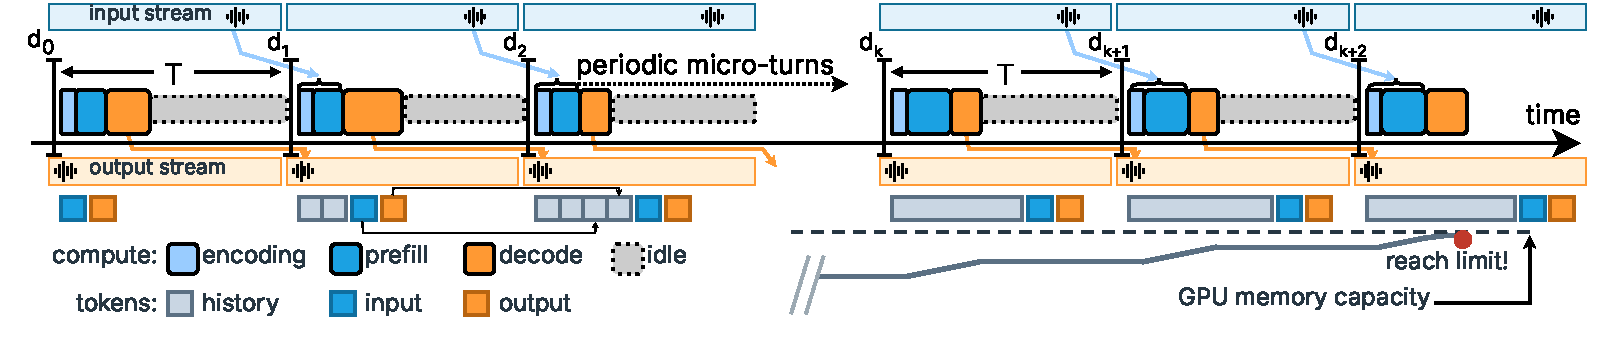
\includegraphics[width=\linewidth]{figures/figure-intro.pdf}
  \caption{Periodic execution with persistent history.
  Each micro-turn encodes and prefills new input and may decode output for playback.
  Retained input and output extend the KV history, which occupies GPU memory even between micro-turns under full residency.
  The timeline and memory growth are schematic, illustrating how retained state can reach the capacity limit.}
  \label{fig:motivation}
  \Description{A periodic session processes input, generates output, and waits for the next period.
  Its retained token history grows, and the corresponding illustrative KV footprint reaches a GPU capacity line.}
\end{figure*}

Retaining less history and offloading idle state make different tradeoffs.
Metronome bounds the KV window of periodic sessions and uses deadline feedback to control admission~\cite{meng2026metronome}.
When an application needs a longer history, offloading idle KV to host memory preserves that history but requires recovery before its next use.
InferCept, for example, chooses among retaining, swapping, and recomputing state for requests paused by external interactions~\cite{abhyankar2024infercept}.
In periodic service, eviction between micro-turns makes recovery a recurring obligation.
Restoring KV only when the next micro-turn arrives delays that micro-turn's computation (Figure~\ref{fig:comparison}(a)).

Periodic execution provides advance notice of when state will be needed again.
The start of each period, or \emph{tick}, is known, so restoration can be scheduled before the next micro-turn.
If the application permits phase assignment, the server can also choose each session's start offset within the period.
Staggering these starts creates opportunities for sessions to reuse GPU space as their state becomes idle.
We call this reuse \emph{memory multiplexing}: each session retains its own history, but its KV need not occupy GPU space throughout the period.

The difficulty is that restoration itself consumes the space that eviction releases.
The server must allocate the entire destination before a copy begins, although the restored KV becomes usable only after the copy finishes.
An early restoration therefore occupies memory that other sessions may still need; a later one has less time to finish before the next tick.
Evicting more KV also increases the time needed to restore it.
The question is how to coordinate session phases, eviction amounts, and restoration times so that transfers finish when needed without exceeding GPU capacity.

\begin{figure}[t]
  \centering
  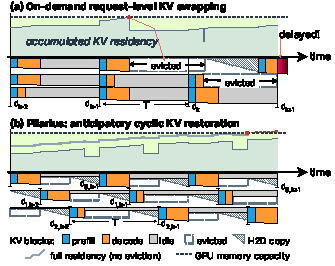
\includegraphics[width=\linewidth]{figures/figure-comparison.pdf}
  \caption{Schematic comparison of restoration timing.
  (a) On-demand swapping delays computation until KV returns.
  (b) Staggered sessions release space for one another's restorations before their next ticks.
  Upper curves show aggregate GPU KV allocation, including each restoration's full destination from the start of allocation.
  Hatching denotes host-to-device (H2D) copies, dotted outlines denote evicted state, and gray denotes idle resident KV.
  The pale curve in (b) shows full residency.}
  \label{fig:comparison}
  \Description{On-demand restoration delays a session, whereas staggered sessions alternate eviction and restoration before their next ticks.
  Aggregate GPU allocation includes the full destination of each ongoing H2D copy.
  A pale curve shows the higher allocation under full residency.}
\end{figure}

We present \systemname, a design for memory multiplexing through \emph{cyclic KV restoration}.
After a micro-turn, \systemname evicts part of the session's idle KV and schedules its restoration to finish by the next tick.
It coordinates these operations across staggered sessions, arranging for space released by one session to accommodate another's restoration (Figure~\ref{fig:comparison}(b)).
The design accounts for both the shared transfer schedule and the GPU space available for each restoration.
Its goal is to increase concurrency while preserving retained history and meeting a recurring soft deadline: each micro-turn should finish by the next tick.

Continued history growth requires planning beyond the current period.
At admission, \systemname considers expected KV growth, computation, transfers, and GPU allocation over a finite lookahead interval.
The resulting plan is reused across micro-turns and revised infrequently as histories grow or sessions enter and leave.
This planning anticipates changes in resource demand; feasibility within the lookahead interval does not guarantee capacity for an entire session.

\placeholder{Final contributions and measured results: identify the configurations where KV capacity limits concurrency while compute time remains; establish the benefit attributable to coordinating phases, eviction amounts, and restoration timing; report concurrency and deadline-miss rates against full residency and on-demand restoration under matched service objectives.}

\section{Background and Motivation}
\label{sec:problem}

\subsection{Periodic Execution and Retained State}
\label{sec:request-classes}
\label{sec:formulation}

A periodic interaction session carries its history from one micro-turn to the next.
The application determines which history to retain, whether through full retention, a fixed window, or a summary.
Residency management changes where the corresponding KV is stored while preserving that choice.
The opportunity to release GPU space depends on when the model uses the state: periodic input capture alone does not establish periodic model execution or an interval without KV accesses.

For timing analysis, consider sessions with a common period $T$ and reference time $t_0$.
Session $i$ has phase $\phi_i\in[0,T)$, so the tick that releases micro-turn $k$ is
\begin{equation}
  r(i,k)=t_0+\phi_i+kT.
  \label{eq:release}
\end{equation}
Each micro-turn should finish generation by the next tick:
\begin{equation}
  c(i,k)\le r(i,k+1)=r(i,k)+T,
  \label{eq:deadline}
\end{equation}
where $c(i,k)$ is generation completion.
This is a soft deadline, with occasional misses allowed under a specified miss-rate limit.
Latency is measured from the planned tick as $c(i,k)-r(i,k)$; delaying input submission or computation does not move the deadline.
Delivery latency and initial phase-alignment delay require separate accounting (Section~\ref{sec:methodology}).
\placeholder{Allowed deadline-miss rate, observation interval, and model-specific generation-completion event.}

Let $q(i,k)$ be the last use of the KV selected for eviction in micro-turn $k$.
That state can leave the GPU once outstanding references are released and a valid host copy is available.
It must return before the next computation accesses it; \systemname targets completion by $r(i,k+1)$ to keep restoration off the next micro-turn's execution path.
The interval from $q(i,k)$ to that tick is the planned window for reclamation and restoration, provided there are no intervening accesses.
Late computation can shorten or eliminate this window.

\subsection{When KV Capacity Limits Concurrency}
\label{sec:capacity-problem}
\label{sec:slack-conditions}

A session's KV-idle interval does not imply spare compute capacity: other sessions may keep the GPU busy throughout it.
Nor do periodic releases alone establish compute slack~\cite{liu1973scheduling}.
The relevant question is whether \emph{all admitted sessions} still leave time within the period when their retained KV fills GPU memory.
Even if each micro-turn adds a predictable amount of state, attention to a growing history can increase execution time.
The memory and compute limits must therefore be compared at the same context length.

Consider a reference configuration with $N$ sessions whose inputs are available at the same tick and whose period is $T$.
Each session reaches a maximum retained length of $L$ positions within the period, with $\kappa$ KV bytes per position and no inter-session sharing.
Let $G_{\mathrm{KV}}$ be the GPU capacity available for KV after weights, activations, and other runtime allocations.
Ignoring allocation rounding, full residency fills this pool at
\begin{equation}
  L_{\mathrm{mem}}=\frac{G_{\mathrm{KV}}}{N\kappa}.
  \label{eq:memory-boundary}
\end{equation}
Let $C_N(L)$ be the elapsed time needed for all $N$ sessions' per-period work under a specified execution policy with the required KV resident.
It includes input processing, model execution, and scheduling overhead; batching means that it is not generally the sum of isolated session times.

The time left at the memory limit is $T-C_N(L_{\mathrm{mem}})$.
To bound it, hold the per-period input and generation work fixed and suppose that, over the context range of interest,
\begin{equation}
  C_N(L)\le A_N+B_NL,\qquad A_N\ge0,\ B_N\ge0.
  \label{eq:compute-envelope}
\end{equation}
The intercept $A_N$ accounts for work independent of history length; the slope $B_N$ allows execution cost to grow with that length.
This affine upper bound is an assumption to establish for the chosen workload, platform, and execution policy.
If $L_{\mathrm{mem}}$ lies in the same range, the remaining time satisfies
\begin{equation}
  T-C_N(L_{\mathrm{mem}})
  \ge T-A_N-\frac{B_NG_{\mathrm{KV}}}{N\kappa}.
  \label{eq:memory-before-compute}
\end{equation}
A positive right-hand side is sufficient for memory to fill before the period's compute budget is exhausted.
If the right-hand side is at least $\eta T$ for $0<\eta<1$, all $N$ sessions leave at least a fraction $\eta$ of the period unused in this reference configuration.

Coefficients fitted to measurements yield a prediction of slack, not a proven lower bound, and require validation on independent configurations.
Even an established slack bound does not show that an additional session or recomputation will meet its deadline: the extra work, recovery costs, and interference must fit while preserving each session's deadline.
\placeholder{Motivating measurement: joint KV allocation and aggregate execution time at the full-residency limit, with concurrency and context length; validate the predicted compute slack on separate configurations.}

\subsection{Restoration Needs Both Time and Space}
\label{sec:opportunity}

Removing a session's KV frees capacity only until the server allocates space to restore it.
The full restoration destination must be allocated before copying starts, even though its KV is not yet usable.
Let $\mathcal{P}(t)$ be the set of physical GPU blocks allocated to KV at time $t$, including destinations of unfinished restorations, and let $b_p$ be the size of block $p$.
A feasible schedule requires
\begin{equation}
  \sum_{p\in\mathcal{P}(t)} b_p \le G_{\mathrm{KV}}
  \quad\text{at every }t,
  \label{eq:memory}
\end{equation}
with each shared physical block counted once.
Counting only valid KV would miss the allocation occupied by ongoing restorations.

That allocation must also occur early enough for the copy to finish.
For a restoration of $e$ bytes starting at time $u$, let $\widehat B$ be its estimated effective host-to-device bandwidth and $\delta$ an allowance for scheduling and completion overhead.
The estimated completion must satisfy
\begin{equation}
  u + e/\widehat B + \delta \le r(i,k+1).
  \label{eq:restore-time}
\end{equation}
The estimate must reflect bandwidth available under the shared transfer schedule, including the effects of host backup traffic and concurrent GPU work, rather than the link's nominal rate.

These constraints pull restoration timing in opposite directions.
An earlier restoration has more time to finish but holds its destination longer; a larger eviction releases more memory but takes longer to restore.
Session phases change when space becomes available and when restored state is needed.
A schedule can consequently fit its total transfer bytes within a period and still fail because transfers overlap or their destinations exceed GPU capacity at some instant.
Memory multiplexing requires checking both the transfer windows and GPU allocation over time, together with computation under the chosen phases.

\section{Problem Formulation}
\label{sec:formulation}

% New file 2026-09-15, hosting docs/PAPER.md §3 (four steps) from
% docs/problem.md workload model and resource frontier.

This section fixes the objects and the objective that design and evaluation
share, so that both use the same verdict.

\paragraph{Sessions and events.}
We model the workload as \emph{periodic interaction sessions}: updates become
eligible on a describable period, and adjacent updates depend on the same
growing history. With a common period $T$ and reference time $t_0$, the $k$-th
update of session $i$ has release time $r(i,k) = t_0 + \phi_i + kT$, where
$\phi_i \in [0, T)$ is the session's release offset. Release means eligibility:
the input is available, not that the request has entered the engine. We
distinguish four events per update: release $r(i,k)$, actual submission
$a(i,k)$, the start $s(i,k)$ of computation that depends on the target KV, and
the completion event $c(i,k)$. The rhythm must come from the workload itself;
a service-stack entrance may choose phase alignment within the application's
contract, in which case $a$ coincides with $r$ in steady state and each
session pays at most one period of alignment wait at its first submission,
reported separately. Waits introduced by deferring ready input count toward
latency, and changes to input chunking must be measured against original input
time.

\paragraph{Service objective.}
The soft real-time objective is $c(i,k) - r(i,k) \le D_i$. The completion
event is the \emph{generation completion} of the update; user-visible delivery
is modeled as a constant offset thereafter, an assumption we state explicitly.
The latency baseline is the actual submission $a(i,k)$ and must be read
together with an update-backlog metric, so that deferred submissions cannot
hide overload. Per-update generation is parameterized as $m(i,k) \le M$. For
sessions with real-time output consumption at rate $R_{\mathrm{play}}$,
bounded buffering and freshness limit how far cumulative generation may lead
consumption: over any $n$ consecutive periods, retained-and-delivered output
obeys $\sum_{j=k}^{k+n-1} N_{\mathrm{out}}(j) \le R_{\mathrm{play}} \cdot nT +
B_{\mathrm{out}}$ for a bounded lead allowance $B_{\mathrm{out}}$. A single
update may emit more than one period of content when prebuffering is allowed;
the contract bounds sustained lead, not each period in isolation.
\placeholder{Concrete target value $D$, permitted violation ratio
(parameterized sweep), observation horizon, and session-failure rule; pending
protocol freeze (measurement semantics owner).}

\paragraph{KV idle intervals.}
Let $q(i,k)$ be the last use of the target KV by update $k$. If the next use
$s(i,k+1)$ starts later and no other execution touches the state, the span
between them is a KV idle interval---the time window in which every
residency-reducing action must fit. For sessions whose bounded update
completes early and whose next update is gated by input and clock, the
interval recurs every period. Periodicity supplies the prediction; queueing,
long computations, backlogged execution, or overlapping access can shorten or
eliminate the interval. Release offsets change how sessions overlap; they
create neither idle time nor bandwidth for any single session.

\paragraph{Resource constraints.}
Physical capacity bounds allocation at every instant: with $G_{KV}$ the usable
KV pool and $b_p$ the size of allocated block $p$, $\sum_{p} b_p \le G_{KV}$,
where prefetch targets count from allocation, before their content arrives.
Peak allocation therefore depends on when eviction and restoration are
scheduled, and allocatable space does not imply content readiness. Treating
the transfer link as a renewable time resource yields a stronger candidate
feasibility condition than aggregate bandwidth checks: each session's periodic
restoration demand should receive enough link time before its deadline. This
condition is a modeling assumption to be calibrated, not a established law:
link time is not exclusively assigned---backup, gap recomputation, and
competing sessions share it---and the window from initiation to completion
includes scheduling waits. One offset assignment thus simultaneously shapes
three coupled resources: link time, the duration of GPU space occupancy, and
batch composition. The same link view bounds the total reclaimable residency
per period by the smaller of the link's per-period byte budget and the total
evictable state, which suggests---again as an assumption to verify---that the
achievable capacity extension is a property of link capability and timing
structure rather than of the per-session retention policy.
\placeholder{Batch-dependent cost function, calibrated transfer service curve,
and the feasibility condition itself; validated by independent calibration and
held-out prediction (Q5).}

\section{System Design}
\label{sec:design}

\subsection{Architecture and Execution Cycle}
\label{sec:design-overview}

\systemname coordinates session phases, eviction budgets, and restoration timing to reuse GPU space between updates.
It operates above an inference backend, which remains responsible for execution scheduling and model computation.
Batch formation, when used, remains a backend policy; the architecture does not require continuous batching.
A residency planner constructs the plan at admission and revises it as resource demands change.
A session manager follows the plan, using ticks, execution events, and KV readiness to submit work to the backend.
A KV memory manager tracks allocation, valid copies, and references, while a KV transfer engine executes asynchronous copies.
The session manager issues eviction and restoration requests to the memory manager, which submits transfer requests with valid sources and allocated destinations.
A transfer completion reports a finished copy; KV readiness is published only after all required ranges are valid for the corresponding session.
These components separate planning decisions from the safe execution of each cycle.

Consider one session in Figure~\ref{fig:motivation}.
At its tick, historical KV is ready on the GPU; the backend processes new input and generates the next output.
Newly retained KV is backed up to host memory.
After the selected ranges are no longer in use and their host copies are valid, \systemname releases their GPU storage.
Other sessions can use this space until the manager allocates a destination and restores the evicted state before the next tick.
Figure~\ref{fig:comparison}(b) shows this cycle across staggered sessions.

\subsection{Session Groups and Phase Assignment}
\label{sec:design-offsets}

\systemname divides a common period $T$ into $S$ phase slots, with release offsets $\phi_j=jT/S$ for $j=0,\ldots,S-1$.
Sessions assigned to the same slot form a session group and become eligible for execution at the same phase.
Each occupied slot can contain multiple sessions; the design does not require one slot per session.
Sessions retain separate histories and eviction budgets, and the backend forms execution batches from the eligible work.
A session group is therefore a scheduling unit, with no requirement that all members execute as one fixed batch or transfer atomically.

\paragraph{Trading batching efficiency for memory reuse.}
Aligning every session to the same phase makes more work available for batching, but also concentrates demand for resident KV and restoration.
Staggering groups distributes that demand and lets their eviction intervals supply space for one another.
It can reduce batch sizes and increase total execution cost through additional model iterations and weight accesses.
Grouping multiple sessions at each phase preserves opportunities for batching while avoiding a single synchronized burst.
For roughly balanced groups, increasing $S$ reduces the number of sessions available per group from $N$ toward $N/S$.
The planner must choose this tradeoff using the backend's measured execution costs.

The goal is to preserve the service target while reducing peak memory use.
Let $C_{\mathrm{aligned}}$ and $C_{\mathrm{grouped}}$ denote the complete periodic execution costs for the two release patterns at the same history length and workload.
The extra cost $C_{\mathrm{grouped}}-C_{\mathrm{aligned}}$, together with transfer interference and scheduling delays, must fit within the original margin $T-C_{\mathrm{aligned}}$.
The short generation bursts described in Section~\ref{sec:request-classes} explain why a moderate batching penalty can leave useful slack.
Admission checks this margin and each session's completion time under the proposed grouping.
Initial phase alignment and any resulting input delay count toward the service cost.

\subsection{Joint Residency Planning}
\label{sec:design-planning}

The planner chooses phase assignments, per-session eviction amounts, and restoration times over a finite lookahead horizon $H$.
It uses the configured period, retained state, expected growth, execution costs under the proposed groups, host capacity, and effective transfer service.
A free phase slot is insufficient for admission: the proposed sessions must fit the compute budget, individual transfer windows, and instantaneous GPU capacity.
Equation~\ref{eq:memory-gain} shows why transfer utilization alone does not establish a capacity benefit; the planner must reduce peak allocation.

\paragraph{Eviction budgets.}
An eviction budget $e_i$ limits the amount of safely recoverable KV released from session $i$.
It need not cover the entire history.
As Section~\ref{sec:opportunity} shows, full eviction eventually exceeds the transfer budget as retained state grows.
Partial eviction keeps the excess resident and gives the planner control over each restoration's duration and destination size.
A useful budget must free enough memory to matter while leaving a feasible return path.

\paragraph{Restoration timing and space.}
Let $r_{i,k+1}$ be the next tick and $u_i$ the planned restoration start.
Given the effective bandwidth assigned to the copy, the estimate $u_i+e_i/\widehat B_i+\delta_i\le r_{i,k+1}$ must include queueing, completion, and safety allowances in $\delta_i$.
The individual estimates must agree with a feasible shared transfer schedule and Equation~\ref{eq:transfer-budget}.
At every point, total physical GPU allocation must remain within $G_{\mathrm{KV}}$.
This accounting includes the entire destination of each copy from the time it is allocated, with shared blocks counted once.
Starting early can shorten the interval of reclaimed space even when it makes the transfer easier to finish.

The planner therefore checks when earlier groups release space as well as when later groups need it.
It must account for expected history growth throughout $H$; a plan that fits the current state may cease to fit before the horizon ends.
\placeholder{Joint planning algorithm: selection of group count and horizon, session assignment, safe eviction ranges, resource estimates and margins, and the time-and-space feasibility check.}

\subsection{Safe Eviction and Scheduled Restoration}
\label{sec:design-idle}
\label{sec:design-correctness}

\paragraph{Backing and releasing state.}
The memory manager incrementally creates host copies of newly retained KV; valid copies of unchanged history can be reused across periods.
Backing up state does not release its GPU allocation.
Eviction requires both a complete host copy and the absence of conflicting execution or transfer references.
For a shared physical block, all references must permit reclamation.
These conditions preserve the application's selected history while changing where its KV resides.

\paragraph{Allocating and copying.}
\label{sec:design-prefetch}
The session manager requests restoration at the planned time.
The memory manager allocates the full destination before submitting a copy to the transfer engine.
Space reclaimed from another group's idle state can satisfy this allocation.
An ongoing copy already occupies GPU capacity, but its contents become usable only after completion is published.
\placeholder{Choose and justify the restoration allocation boundary: whole-group reservation or per-session allocation under the group schedule; specify readiness and recovery when a later allocation cannot proceed.}

\paragraph{Resuming computation.}
The backend may access restored KV only after all required ranges are valid for the correct session and logical positions.
Concurrent demand, prefetching, and eviction must share a consistent view of allocation and content validity.
If space or transfer service is unavailable at the planned time, the manager must reassess completion before allowing dependent computation.
Demand restoration can recover missing state, but its delay remains part of service latency and can cause a deadline miss.
No timeout permits reading unfinished KV or reusing a referenced block.

\subsection{Plan Reuse and Revision}
\label{sec:design-revisions}

The planner reuses its plan across updates when state growth remains sufficiently predictable over the horizon.
Per-cycle checks enforce current space, reference, and readiness conditions without reselecting every phase and budget.
Accumulated history growth requires infrequent revisions; session arrivals and departures can require larger adjustments.
Keeping some KV resident limits transfer traffic, but that resident portion can still grow and eventually exhaust the available capacity.

Revisions must account for allocations and transfers already in progress.
A new plan cannot release a referenced block or turn an unfinished copy into valid state.
Feasibility within $H$ therefore supports only that planning horizon, with continued service requiring reassessment.
\placeholder{Revision triggers, horizon extension, transition between plans with in-flight work, and service policy when no feasible revision exists.}

% Included after System Design; this is a subsection of that section.
\subsection{Backend Integration}
\label{sec:implementation}

The backend interface must expose request submission, execution completion, KV block identity, allocation, references, and copy readiness.
\systemname coordinates these operations with the backend's existing block allocator so that memory accounting and validity have one consistent authority.
The backend controls execution scheduling and any batching policy; session groups determine which work becomes eligible together.
\placeholder{Verified integration: identify the backend and implemented planning and recovery paths, synchronization points, and remaining gaps relative to this design.}

\section{Evaluation Methodology}
\label{sec:methodology}

% Rebuilt 2026-09-15 from docs/PAPER.md §6① and docs/experiments.md
% (comparison families, fairness, ablation matrix, measurement semantics).

Our evaluation is organized around seven questions: whether KV capacity limits
service before compute or input handling does (Q1); how many sessions each
system can serve within the objective (Q2); at what latency cost (Q3); what
each mechanism contributes (Q4); whether the resource model predicts held-out
operating points (Q5); whether state round-trips preserve retained semantics
(Q6); and where the approach stops helping (Q7).

\paragraph{Fairness.}
Formal comparisons fix the model and precision, input content and processing
semantics, actually executed generation work, reference history, scheduling
mode, batching budgets, cache and host-copy budgets, output-delivery
accounting, and observation switches. End-to-end comparisons must match work
and apply a uniform service verdict; claims that a specific mechanism causes a
benefit must control variables. Configuration names and default switches do
not substitute for verifying the executed path.

\paragraph{Compared systems.}
The comparison families are: full residency (the reference policy, and the
capacity and latency baseline), recomputation of missing state, on-demand host
reload, \systemname and its ablations, the closest session-level KV-management
systems, and retention policies such as windowing or summarization---the last
included as workload parameters that change per-session retained-state size,
not as baselines to defeat, and without adjudicating quality among retention
policies.
\placeholder{Selection and adaptation of the closest external systems
(candidates include session-KV tiering and duplex-serving systems); versions,
missing capabilities, and re-implementation status to be documented.}

\paragraph{Ablations and the three grades of timing.}
Restoration-trigger arms map to the three grades of timing information:
on-demand restoration and post-submission prefetch use no future timing;
rhythm-based prefetch uses the first two grades (rhythm and visible release
times); the release-policy arm (aligned versus staggered offsets) tests the
third grade, offset control. Reference history, host copies, and the transfer
path are held fixed across arms, and the actual moment each trigger signal is
produced is recorded. An oracle arm with exact future information, if used, is
labeled as an undeployable upper reference.

\paragraph{Metrics.}
Update service latency runs from actual submission $a(i,k)$ to generation
completion, with each session's one-time alignment wait reported separately,
and is always read together with the update-backlog metric. Capacity is
reported as offered, admitted, and completed load under the stated deadline,
distribution, and horizon. KV occupancy separates allocated space, valid
content, reusable cache, and host copies; restoration cost separates bytes,
initiation queueing, transfer, completion reporting, and rescheduling wait.
Sustained growth makes the workload non-stationary, so trajectories over time
and context are reported rather than single steady-state points.
\placeholder{Workload and platform instantiation: application timing
contracts, session-lifetime distributions, retention-policy parameters, state
geometry, and device/interconnect inventory; the matrix is not yet frozen and
no current prototype configuration is promoted to paper scope.}

\section{Evaluation}
\label{sec:evaluation}

% Rebuilt 2026-09-15 from docs/PAPER.md §6②–⑦. Every result is a placeholder;
% interpretation rules are pre-registered so results cannot be re-scoped after
% the fact.

\subsection{When Does KV Capacity Bind?}
\label{sec:eval-capacity-bound}

Sweeping concurrency and context length while jointly observing KV allocation,
model progress, queueing, and compute tests whether a KV-capacity-bound region
exists---the proposition behind Figure~\ref{fig:tension}.
\placeholder{Q1 result: measured region where KV allocation limits admitted
service while compute and input handling retain slack; if input processing or
compute always saturates first, the capacity motivation does not hold in the
studied domain and the paper's claims contract accordingly.}

\subsection{Capacity and End-to-End Service}
\label{sec:eval-main}

Under the uniform service verdict we compare the admitted load of full
residency, on-demand restoration, and \systemname.
\placeholder{Q2 main result: sessions served within the objective per system,
with offered/admitted/completed accounting and service distributions under
equal load. Interpretation is pre-registered: higher within-objective
admission supports the core claim; lower residency without higher admission
contracts the conclusion to ``residency saved, no service benefit.''}

\subsection{Latency Cost and the Critical Path}
\label{sec:eval-latency}

\placeholder{Q3 result: input-to-result distributions and the restoration
critical path decomposed into submission, transfer, completion reporting, and
rescheduling. Interpretation: quantified costs that do not cancel the capacity
benefit support the design; violations from latency or sustained backlog
shrink the validity domain.}

\subsection{Mechanism Analysis}
\label{sec:eval-ablation}

\placeholder{Q4 ablations: offsets, host copies, eviction, post-submission
versus rhythm-based prefetch, and their interactions, with reference history,
host copies, and transfer paths fixed. Interpretation: benefits that grow with
the grade of timing information support ``timing itself has value''; benefits
traced to unmatched generation or execution modes void the affected arm.}

\subsection{Resource Model Validation}
\label{sec:eval-model}

\placeholder{Q5 result: independent calibration, held-out prediction of
bottleneck class and error, and reported failure points. Interpretation:
correct held-out prediction qualifies the resource model as a contribution;
point-wise refitting demotes it to an analysis tool.}

\subsection{Correctness}
\label{sec:eval-correctness}

\placeholder{Q6 result: state round-trip consistency against reference
execution and retained-history preservation, under the same standard for all
systems. Interpretation: consistent round-trips support the claim that the
mechanisms are transparent to the reference execution; inconsistency or input
loss contracts the correctness claim.}

\subsection{Overheads, Boundaries, and Failure}
\label{sec:eval-limits}

\placeholder{Q7 result: overheads and failure regions under short sessions,
late input, coverage gaps, bandwidth and host-capacity pressure, reported
without deleting failed regions from the main figures.}

\section{Related Work}
\label{sec:related-work}

\draftplaceholder{Complete planning/related-work-matrix.md before writing prose. Compare capabilities and assumptions, not just publication summaries.}

\subsection{Interactive and Streaming Model Serving}

\subsection{KV Cache Management and Tiering}

\subsection{Real-Time and Periodic Scheduling}

\section{Discussion and Limitations}
\label{sec:discussion}

\draftplaceholder{State applicability boundaries, resource-regime transitions, workload assumptions, unsupported modalities, and operational failure modes without overgeneralizing from the measured stack.}

\section{Conclusion}
\label{sec:conclusion}

\draftplaceholder{Restate the supported problem, mechanism, and result in three to five sentences. Do not add a new claim here.}


\bibliographystyle{ACM-Reference-Format}
\bibliography{references}

\end{document}
